\section{Dabiskās valodas apstrāde}
Dabiskās valodas apstrāde (angliski – natural language processing jeb NLP) ir daudznozaru joma, kas apvieno lingvistikas, datorzinātnes un mašīnmācīšanās elementus, lai ļautu datoriem saprast, interpretēt un ģenerēt cilvēka valodu. 

DVA sastāv no vairākām pamata komponentēm:
\begin{itemize}
\item Tokenizācija: teksta sadalīšanas process vārdos vai frāzēs (tokenos)
\item Morfoloģiskā marķēšana: gramatikas marķējumu piešķiršana vārdiem
\item Sintakses parsēšana: teikumu gramatiskās struktūras analīze
\item Nosaukto entitāšu atpazīšana: nosaukumu atpazīšana un kategorizācija, piemēram, personvārdi, datumi un atrašanās vietas
\item Lemmatizācija: vārdu pārveidošana pamatformā
\end{itemize}

Pielietojot daļu no šīm komponentēm tālāk iespējami sarežģītāki pielietojumi teksta apstrādei – kategorizācijai, noskaņojuma analīzei, mašīntulkošanai, čatbotu izveidei. 

Sākotnējās DVA sistēmas balstījās uz manuāli izstrādātām noteikumiem, taču šīs sistēmas ir ierobežotas ar savu nespēju apstrādāt cilvēka valodas daudzveidību un sarežģītību, kā rezultātā DVA sistēmas mūsdienās bieži tiek veidotas tieši ar mašīnmācīšanās iesaisti.

\section{Mašīnmācīšanās}
Mašīnmācīšanās ir mākslīgā intelekta nozare, kas nodarbojas ar datorprogrammu izstrādi, kuras, izmantojot algoritmus un statistikas modeļus, mācās no datiem un uzlabo savu precizitāti. Toms Mičels savukārt apraksta mašīnmācīšanās jomu, izvirzot centrālo jautājumu, ko tā pēta: "Kā mēs varam izveidot datoru sistēmas, kas automātiski uzlabojas, iegūstot pieredzi, un kādi ir pamatlikumi, kas nosaka visus mācīšanās procesus?" \cite{definitionML}.

Induktīvā mācīšanās ir mašīnmācīšanās apakšnozare, kas specifiski nodarbojas ar modeļu mācīšanos no novērojumiem. Šajā nozarē mācīšanās uzdevumi bieži tiek raksturoti, pamatojoties uz atgriezenisko saiti, kas tiek sniegta apmācības veicējam \cite{russel2010}, šādi:

\begin{itemize}
\item Uzraudzīta mācīšanās: Apmācības procesā tiek sniegts vēlams izvads katram novērojumam. Mērķis ir iemācīties funkciju, kas paredz pareizo izvades vērtību brīdī kad tiek sniegts iepriekš neredzēts novērojums.
\item Neuzraudzīta mācīšanās: Apmācības laikā netiek sniegts izvads. Mērķis ir atklāt paraugus un regulāras iezīmes datos.
\item Stimulētā mācīšanās: Šis ir īpašs uzraudzītās mācīšanās gadījums, kur apmācības posmā tiek sniegta atlīdzība pēc katras darbības.
\end{itemize}

Uzraudzītas mācīšanās gadījumus, kad uzdevums ir iemācīties diskrēti vērtētu funkciju, sauc par klasifikāciju. Uzdevums, kad jāiemācās nepārtraukti vērtēta funkcija, tiek saukts par regresiju. Savukārt klasterošana ir neuzraudzītās mācīšanās uzdevums, kas atrod līdzīgu objektu grupas datu kopā.

\section{Tekstu klasifikācija}

Teksta klasifikācijas mērķis ir tekstu piesaiste konkrētai kategorijai, balstoties uz teksta saturu. Šāda klasifikācija ir ļoti izplatīta ziņu portālos un citur, kur nepieciešams kategorizēt lielu rakstu daudzumu, piemēram akadēmisko darbu datubāzēs. Mašīnmācīšanās algoritmi ļauj rast risinājumu automātiskai šādu tekstu kategorizēšanai un daudzām citām klasifikācijas problēmām, piemēram, ar augstu precizitāti noteikt vai ienākošais e-pasts ir vai nav mēstule. Iespējams arī veikt sentimentu analīzi un noteikt cilvēku attieksmi par kādu konkrētu tematu, piemēram, M. Kandias ir apskatījis kā ar tekstu klasifikācijas palīdzību noteikt negatīvu attieksmi pret likumsargiem, balstoties uz konkrēta lietotāja ierakstiem vietnē YouTube \cite{threatdetectionyoutube}.

\begin{figure}[H]
	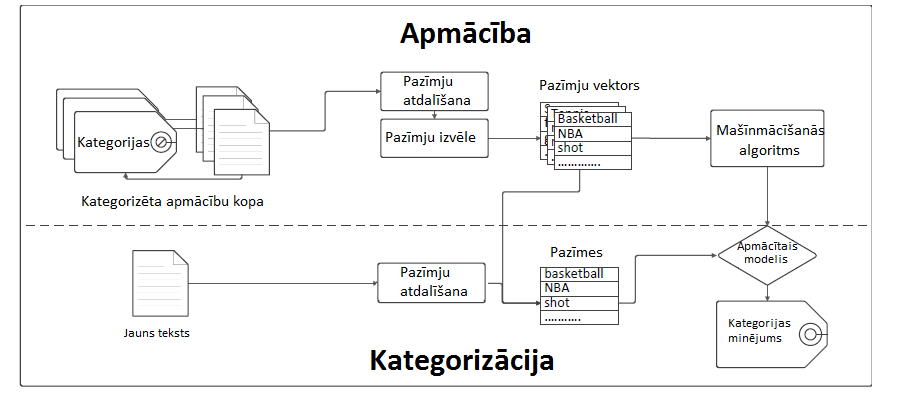
\includegraphics[width=\textwidth]{masinmacisanas}
	\caption{Mašīnmācīšanās tekstu klasifikācijai}
	\label{fig:masinmacisanas}
\end{figure}

Teksta klasifikācijas piemēru ar mašīnmācīšanās pielietojumu iespējams redzēt attēlā  \ref{fig:masinmacisanas}. Pieņemsim, ka dota datu kopa ar sporta ziņām, un risināmā problēma ir - kā klasificēt jaunu dokumentu, piešķirot tam atbilstošā sporta veida kategoriju. Sākumā būs nepieciešami apmācības dokumenti (ar klases marķējumiem) no kuriem mācīties. Tālāk katru ziņu mēs pārveidojam par pazīmju kopu, kuru vektorizētā veidā mēs varam padot tālāk mašīnmācīšanās algoritmam. Ar šo informāciju algoritms izveido modeli, kas var paredzēt iepriekš neredzētu tekstu kategoriju.

\subsection{Klasiskie algoritmi tekstu klasifikācijai}

\subsubsection{Naivā Bejesa metode}
Naivā Bejesa  mašīnmācīšanās algoritms bieži tiek lietots tieši klasifikācijas uzdevumos tā veiktspējas un efektivitātes dēļ.  Tas balstās uz Bejesa teorēmu, kas ir viena no pamatteorēmām varbūtību teorijā. Šī teorija apraksta notikuma varbūtību, pamatojoties uz iepriekš zināmiem datiem. Teksta klasifikācijas kontekstā teorēma palīdz mums aprēķināt varbūtību dokumenta piederībai noteiktai klasei.

Bejesa teorēmu var izteikt šādi:
\begin{equation} \label{naivebayes}
   P(klase|dokuments) = \frac{P(klase) \cdot P(dokuments|klase)}{P(dokuments)}
\end{equation}

 Kur formulā \ref{naivebayes}:
\begin{itemize}
\item \(P(klase|dokuments)\) ir varbūtība, ka dokuments pieder norādītajai klasei.
\item \(P(klase)\) ir apriorā klases varbūtība.
\item \(P(dokuments|klase)\) ir varbūtība novērot dokumentu, zinot klasi.
\item \(P(dokuments)\) ir varbūtība, ka dokuments parādās datu kopā.
\end{itemize}

"Naivais" aspekts Naivajā Bejesā nāk no pieņēmuma, ka pazīmes (vārdi tekstā) ir neatkarīgas. Citiem vārdiem sakot, mēs pieņemam, ka katra vārda klātbūtne vai neesamība dokumentā ir neatkarīga no citu vārdu klātbūtnes vai neesamības. Šis ir vienkāršs pieņēmums, bet tāds kurš bieži darbojas praksē.

\subsubsection{Loģistiskā regresija}

Loģistiskā regresija modelē varbūtību, ka dokuments pieder konkrētai klasei, izmantojot loģistisko (sigmoidālo) funkciju \cite{WITTEN201185}, kas nodrošina, ka izvades varbūtība ir starp 0 un 1. Loģistiskā funkcija tiek definēta šādi:
\begin{equation} \label{formula1}
 P(y=1|x) = \frac{1}{1 + e^{-z}}\
\end{equation}
Kur formulā \ref{formula1}  \(P(y=1|x)\)  ir varbūtība, ka dokuments pieder klasei 1 un  \(z\) ir lineāra kombinācija no ievades iezīmēm un modeļa parametriem.
Lineāra kombinācija tiek aprēķināta šādi:
\begin{equation} \label{formula2}
   z = \theta_0 + \theta_1 x_1 + \theta_2 x_2 + \ldots + \theta_n x_n
\end{equation}
Kur formulā \ref{formula2}  \(x_1, x_2, \ldots, x_n\) ir skaitliskās iezīmes, kas izgūtas no teksta dokumenta un \(\theta_0, \theta_1, \ldots, \theta_n\)  ir modeļa parametri, arī saukti par svariem vai koeficientiem.

Apmācības fāzē loģistiskās regresijas modelis mācās optimizēt savus parametrus (\(\theta\)) no marķētajiem datiem, lai iegūtu pēc iespējas pareizākus minējumus.

\subsubsection{Lēmumu koki}

Lēmumu koka klasifikators izmanto koka modeli, lai prognozētu teksta klasi. Koks sastāv no viena saknes mezgla, kas ir uzskatāms par klasifikatora sakuma punktu. Pārējie mezgli ir lapu mezgli, ja tiem nav zaru, vai iekšējie mezgli. Iekšējie mezgli un saknes mezgls ir iezīme un pārbaude, kas jāveic šai iezīmei. Katrs iespējamais testa rezultāts ir mezgla atzars, kas ved uz nākamo mezglu. Šādi veicot pārbaudes uz katra mezgla, tiek iziets caur visiem mezgliem līdz pirmajam lapu mezglam. Lapu mezgli galu galā norāda uz klasi, kurai šis teksts pieder. Citiem vārdiem – klase tiek paredzēta, sekojot ceļam no koka saknes mezgla, līdz tas saskaras ar lapas mezglu \cite{mitchell1997}. 

Apmācības algoritma mērķis šajā gadījumā ir izveidot lēmumu koku, pamatojoties uz apmācību datu piemēriem. Tomēr algoritmam ir jāizvairās veidot koku, kas pārmērīgi atbilst apmācības datiem. Tāpēc optimālais koks ir mazākais lēmumu koks, kas vislabāk atšķir klases.

\begin{figure}[H]
	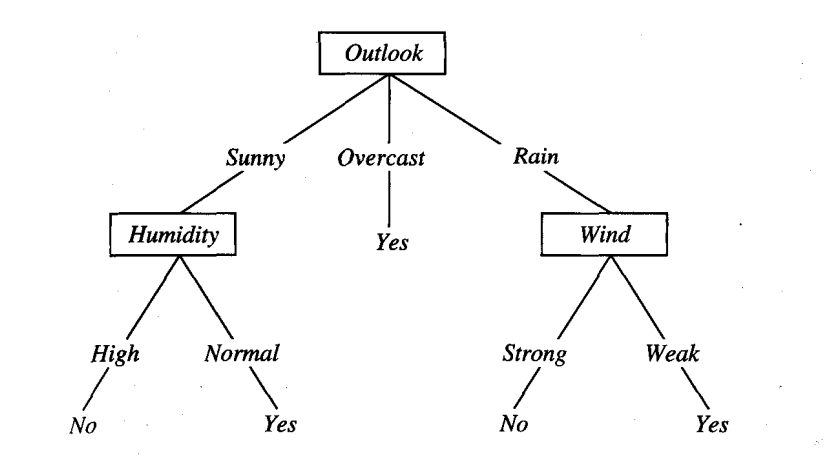
\includegraphics[width=\textwidth]{lemumu_koks_teorija}
	\caption{Lēmumu koka ilustrācija \cite{mitchell1997} }
	\label{fig:lemumu_koks_teorija}
\end{figure}

Piemērā \ref{fig:lemumu_koks_teorija} apskatām vienkāršu šāda koka reprezentāciju, kur veicam klasifikāciju par to vai šis ir piemērots laiks tenisa spēlei ārpus telpām. Ar ieejas datiem kā laikapstākļi (outlook) – saulaini (sunny), mitrums (humidity) – augsts (high), mēs virzītos pa mezgliem “Laikapstākļi”, “Mitrums” līdz lapas mezglam kurš klasificētu laiku kā nepiemērotu tenisa spēlei.

\subsubsection{Atbalsta vektoru mašīnas (SVM)}

Atbalsta vektora mašīnas \cite{supportvectornetworks} (angliski - support vector machines jeb SVM) ir pārraudzītās mācīšanās algoritms kurš ir diezgan populārs tieši klasificēšanas problēmu risināšanā. Šis algoritms veic klasifikāciju konstruējot n-dimensiju hiperplakni kura optimāli ierobežo datus divās nošķirtās kategorijās. Lai vieglāk ilustrētu algoritma darbību, varam apskatīt divdimensiju piemēru.
\begin{figure}[H]
	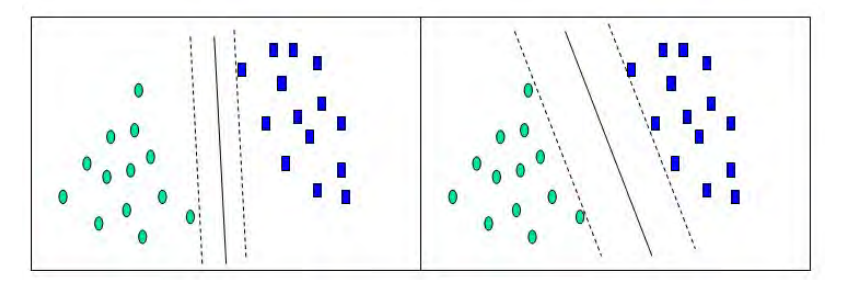
\includegraphics[width=\textwidth]{svm1}
	\caption{Atbalsta vektora mašīnas algoritma ilustrācija \cite{supportvectornetworks} }
	\label{fig:svm1}
\end{figure}
Šajā piemērā \ref{fig:svm1} gadījumi ar vienu kategoriju atrodas pa kreisi (apzīmēti ar zaļiem apļiem) un ar otru kategoriju – pa labi (apzīmēti ar ziliem kvadrātiem). Atbalstu vektora mašīnas analīze mēģinās atrast 1-dimensijas hiperplakni (līniju) kura atdala datus balstoties uz kategoriju kurai tie pieder. Ir praktiski neierobežots līniju skaits, kas spētu veikt šādu nodalījumu, attēlā norādīti 2 piemēri un atliek gūt atbildi uz jautājumu – kura līnija ir labāka kategorizācijas veikšanai vispārīgā gadījumā. Raustītās līnijas, kuras zīmētas paralēli atdalošajai līnijai, iezīmē attālumu starp atdalošo līniju un tai tuvāko vektoru. Šo attālumu sauc par robežu (angliski – margin). Vektori kas atrodas pie šīs robežas ir atbalsta vektori.
\begin{figure}[H]
	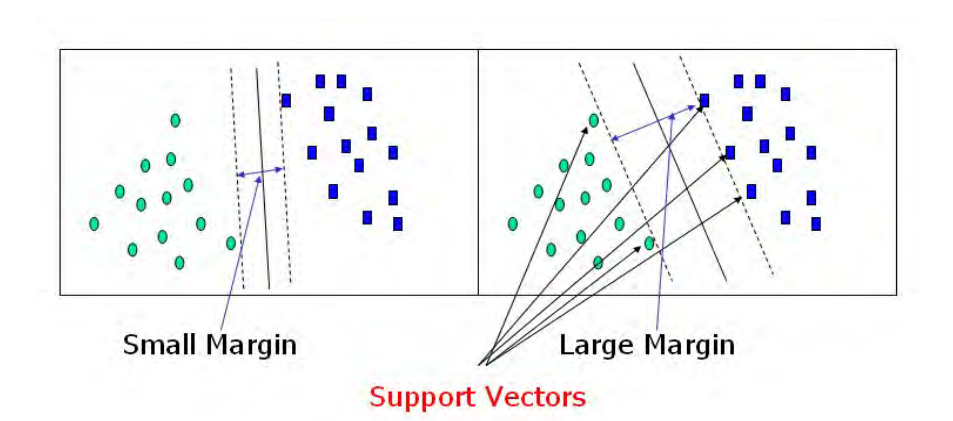
\includegraphics[width=\textwidth]{svm2}
	\caption{Robežas un atbalsta vektoru ilustrācija \cite{supportvectornetworks} }
	\label{fig:svm2}
\end{figure}
Atbalstu vektora mašīnas analīze atradīs līniju (vispārīgi – hiperplakni), kas novietota pēc iespējas lielāku robežu starp atbalsta vektoriem.

\subsection{Neironu tīkli}
Cilvēka smadzenes ir neironu tīkla arhitektūras iedvesmas avots. Cilvēka smadzeņu šūnas, ko sauc par neironiem, veido sarežģītu, savstarpēji cieši saistītu tīklu, kurā neironi sūta viens otram elektriskus signālus ar mērķi palīdzēt cilvēkiem apstrādāt informāciju. Līdzīgi mākslīgais neironu tīkls ir veidots no mākslīgiem neironiem, kas strādā kopā, lai atrisinātu problēmu \cite{AwsNeuralNetworks}. 

Sākumā jāapskata māklīgā neironu tīkla pamatvienība - neirons.
\begin{figure}[H]
	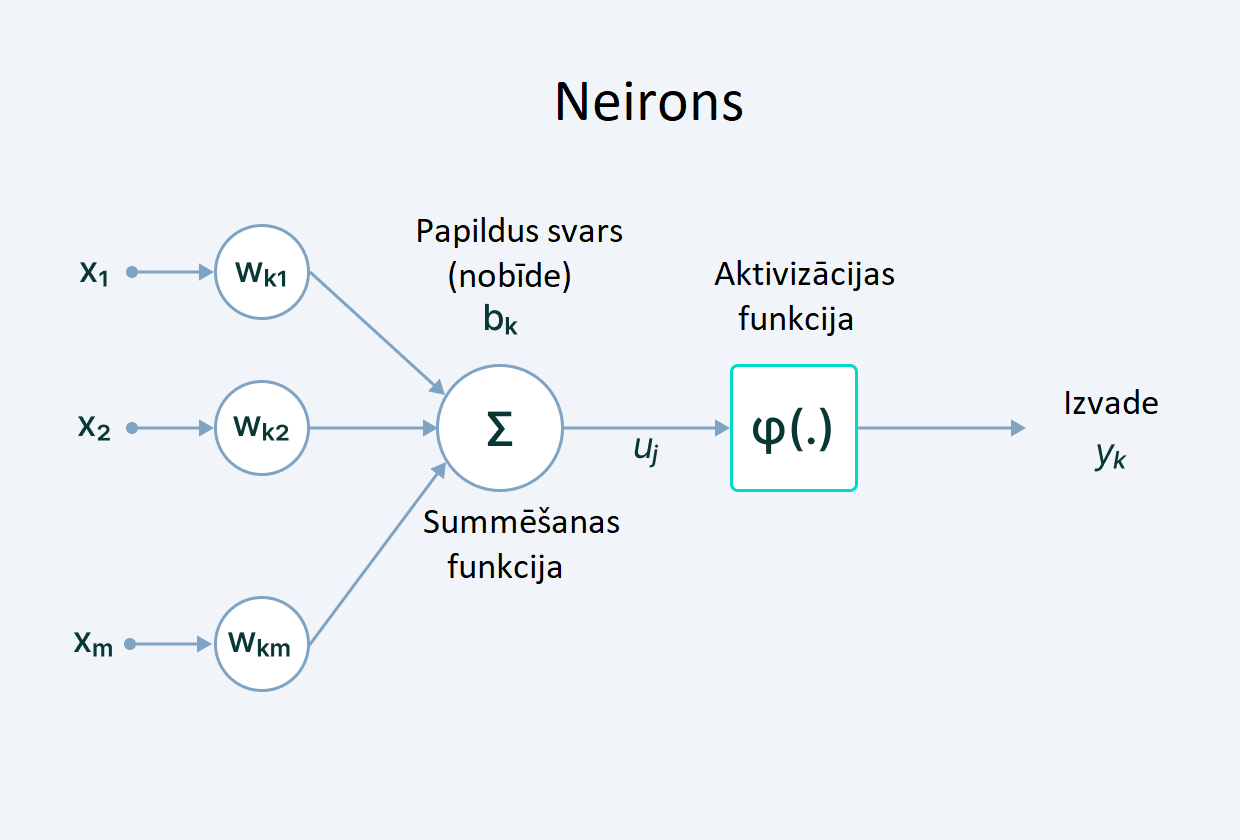
\includegraphics[width=\textwidth]{neirons}
	\caption{Mākslīgā neirona attēlojums}
	\label{fig:neirons}
\end{figure}

Kā redzams attēlā attēlā \ref{fig:neirons}, šī neirona uzbūvi raksturo tā 4 pamatelementi - ieejas signāls, svars, summēšanas funkcija, aktivizācijas funkcija un nobīde.

Ieejas signāls - tas ir neironā ienākošais signāls. Izcelsme tam var būt ārēja vai arī tas var būt cita neirona izejas signāls. Šādi ieejas signāli neironam var būt vairāki.

Svars - tā galvenā funkcija ir piešķirt tiem ieejas signāliem, kas ir svarīgas pareizam problēmas risinājumam. Piemēram, negatīvs vārds ietekmētu noskaņojuma analīzes modeļa lēmumu vairāk nekā neitrālu vārdu pāris. Svara vērtības tiek noteiktas apmācības procesā.

Summēšanas funkcija - šīs funkcijas mērķis ir apvienot vairākus ieejas signālus un to svarus vienā vērtībā, ko tālāk padot aktivizācijas funkcijai.

Aktivizācijas funkcija - šī funkcija izrēķina aktivitātes stāvokli, kas bieži ir arī neirona izejas vērtība.	

Papildus svars (novirze) -  novirzes uzdevums ir novirzīt aktivizācijas funkcijas radīto vērtību. Tās loma ir līdzīga konstantes lomai lineārā funkcijā un gluži kā svars tā vērtība tiek noteikta apmācībnas procesā.

Kad vairāki neironi ir salikti kopā pēc kārtas, tie veido slāni. Vairākus slāņus apvienojot varam iegūt daudzslāņu neironu tīklu. Vienkārša daudzslāņu neironu tīkla arhitektūra aprakstāma kā savstarpēji savienoti mākslīgie neironi trīs slāņos.

\textbf{Ievades slānis}

Informācija no ārpasaules caur ievades slāni nonāk mākslīgajā neironu tīklā. Ievades mezgli apstrādā datus, analizē vai klasificē tos un nodod tos nākamajam slānim.

\textbf{Slēptais slānis}

Slēptie slāņi izmanto ievadi no ievades slāņa vai citiem slēptiem slāņiem. Mākslīgajiem neironu tīkliem var būt liels skaits slēpto slāņu. Katrs slēptais slānis analizē iepriekšējā slāņa izvadi, apstrādā to tālāk un nodod nākamajam slānim.

\textbf{Izvades slānis}

Izvades slānis sniedz visu mākslīgā neironu tīkla veiktās datu apstrādes gala rezultātu. Tam var būt viens vai vairāki mezgli. Piemēram, ja mums ir bināra (jā/nē) klasifikācijas problēma, izvades slānim būs viens izvades mezgls, kas dos rezultātu 1 vai 0. Tomēr, ja mums ir vairāku klašu klasifikācijas problēma, izvades slānis var sastāvēt no vairāk nekā viena izvades mezgla.

\section{Modeļu novērtēšana un validācija}
Pēc apmācīta modeļa iegūšanas ir svarīgi novērtēt izveidotā modeļa veiktspēju un to, cik labi tas spēs veikt tekstu klasifikāciju ar jauniem datiem. 
Viena no izplatītākajām novērtēšanas metodēm ir metode ar noturēšanu (holdout method), kur paraugu kopa tiek sadalīta divās daļās – apmācības kopa un testa kopa. Klasifikators tad tiek apmācīts ar apmācību kopu un validēts ar testa kopu. Šīs metodes mīnuss ir tas, ka apmācībai pieejama mazāka datu kopa. Cita negatīvā īpašība šai metodei ir arī tā, ka rezultāti ir atkarīgi no nevienlīdzīgā datu sadalījuma starp šīm abām kopām.

Cita metode ir nejauša paraugu atlase (Random Subsampling). Šī metode atkārto metodi ar noturēšanu vairākas reizes, lai labāk noteiktu modeļa veiktspēju, tomēr arī šai metodei piemīt pirmās metodes negatīvās īpašības.
Modeļa novērtēšana ar apmācību datiem nav ieteicama, jo tādējādi notiks pārmērīga pielāgošana (overfitting) un mašīnmācīšanās modelis iegaumēs apmācības datus, bet nespēs pareizi klasificēt jaunus datus.

Visbeidzot var izmantot arī šķērsvalidāciju (cross-validation). Šī metode sadala paraugu kopu k vienādās daļās un izmanto katru no šīm daļām tieši vienu reizi priekš testēšanas  Citas, k-1, reizes katra daļa tiek izmantota apmācībai.

\subsection{Klasifikācijas mēri}
\renewcommand{\theequation}{2.\arabic{equation}}
Klasifikācijas problēma ir bieži apskatīts mašīnmācīšanās temats un visizplatītākie mēri, ar kuriem novērtēt modeļa precizitāti ir aprakstīti zemāk.

\subsubsection{Pārpratumu matrica}
Pārpratumu matrica ļauj pārredzami attēlot modeļa precizitāti modelim ar 2 un vairāk klasēm. Matrica sastāv no 2 asīm, kur uz x ass tiek attēlotas visas klases un uz y ass tiek attēloti klases minējumi. Katra matricas šūna satur minējumu skaitu attiecīgajai klases un minētās klases kombinācijai.

Bināras klasifikācijas gadījumā pārpratumu matrica varētu būt attēlojama ar šādu tabulu:
\begin{table}[H]
\centering
\caption{\label{tab:novertejums}}
\textbf{Pārpratuma matrica\\}
\begin{tabular}{|l|l|l|}
\hline
  & +  & -  \\ \hline
+ & PA & KA \\ \hline
- & KN & PN \\ \hline
\end{tabular}
\end{table}

Kur tabulas  \ref{tab:novertejums} vērtības raksturojamas šādi:
\begin{itemize}
\item PA - pareiza atbilsme (tabulā - gadījumi, kad '+' tiek pareizi klasificēts)
\item PN - pareiza neatbilsme (tabulā - gadījumi, kad '-' tiek pareizi klasificēts)
\item KA - kļūdaina atbilsme (tabulā - gadījumi, kad '-' tiek nepareizi klasificēts kā '+')
\item KN - kļūdaina neatbilsme (tabulā - gadījumi, kad '+' tiek nepareizi klasificēts kā '-')

\end{itemize}
\subsubsection{Akurātums}
Akurātums ir mērs, kurš norāda cik no minējumiem ir bijuši pareizi. Tas ir pareizo minējumu dalījums ar visu minējumu skaitu.
\begin{equation}
Akur\bar{a}tums = \frac{PA + PN}{PA + PN + KA + KN}
\end{equation}
\subsubsection{Precizitāte}
\begin{equation}
Precizit\bar{a}te = \frac{PA}{PA + KA}
\end{equation}
\subsubsection{Pārklājums}
\begin{equation}
P\bar{a}rkl\bar{a}jums = \frac{PA}{PA + KN}
\end{equation}
\subsubsection{F1 mērs}
F1 mērs ir precizitātes un pārklājuma mēru harmoniskais vidējais.
\begin{equation}
F1 = \frac{(2 * precizit\bar{a}te * p\bar{a}rkl\bar{a}jums)}{(precizit\bar{a}te + p\bar{a}rkl\bar{a}jums)}
\end{equation}
Atšķirībā no aritmētiskas vidējās vērtības, harmoniska vidējā vērtība tiecas uz mazāko vērtību no diviem mēriem, no tā izriet, ka F1 mērs būs zems ja precizitāte vai pārklājums ir zems.

\section{Tekstu priekšapstrādei}
Pirms iespējams izveidot klasifikācijas modeli, DVA problēmvidē nepieciešams veikt teksta priekšapstrādi, lai dati būtu pielietojami tālākā apstrādē. Tas sevī ietver gan dažādu teksta fragmentu atmešanu, gan pārveidošanu formā kuru spētu saprast apmācIbas algoritmi. Tālāk apskatīti konkrēti priekšapstrādes soļi.

\subsection{Vārdu atdalīšana}
Lai tekstu izmantotu klasificēšanā, ir jāspēj atdalīt atsevišķas šī teksta daļas. To iespējams paveikt dažādos veidos – tekstu iespējams sadalīt pa individuāliem vārdiem vai arī  secīgu vārdu grupām. Vārdu atdalīšanai var izmantot dažādus atdalošos simbolus, piemēram atstarpi un jaunas līnijas sākuma simbolu (\textbackslash n’). Tomēr ne visi atdalošie simboli ir viennozīmīgi, piemēram punkts var būt gan kā teikuma beigas, gan kā daļa no konkrētas vērtības (skaitlis 10.5).
Vārdu atdalīšana secīgās vārdu grupās izmanto n-grammas, kas ir n secīgu vārdu un/vai simbolu kopa tekstā. Izmantojot n-grammas, iespējams iegūt plašāku teksta kontekstu no atdalītajiem vārdiem.

\subsection{Sakņu atdalīšana un lemmatizācija}
Apstrādājot tekstus, svarīgi ir arī ņemt vērā faktu, ka dažādos tekstos viens un tas pats vārds bieži tiek lietots dažādos locījumos un visbiežāk locījumam nav ietekme uz to vai teksts pieder konkrētai kategorijai vai nē. Svarīgi arī ņemt vērā, ka liels individuālo vārdu atkārtojums dažādos locījumos palielina klasifikācijai nepieciešamo laiku un resursus. Sakņu atdalīšana un lemmatizācija risina šo problēmu, pārvēršot vārdus to pamatformā. 

\subsection{Stopvārdu dzēšana}
Bieži vien noderīga ir arī tā sauktā stopvārdu (angliski - stopwords) dzēšana no apstrādāmajiem datiem. Tie ir vārdi kuri neietekmē teksta saturu un to biežais lietojums var atstāt negatīvu ietekmi uz klasifikācijas akurātumu. Latviešu valodā piemērs šādiem vārdiem būtu palīgvārdi, kuri tiek saprasti kā saikļi (un, bet, vai u.c.), prievārdi (uz, no u.c.), partikulas (arī, diezin, gan u.c.).

\subsection{Vektorizācija}
Teksta vektorizācija ir process, kurā teksta informācija tiek pārveidota skaitļu formā, ko tālāk savukārt var izmantot mašīnmācīšanai. Šis solis ir būtisks, jo lielākā daļa mašīnmācīšanās algoritmu strādā ar skaitļiem, bet teksta dati ir paši par sevi neskaitliski. Teksta vektorizācijai ir vairākas metodes, populārākās no tām uzskaitītas zemāk.

\subsubsection{Vārdu maiss}
Vārdu maiss – tā ir nesakārtota vārdu kopa, kur vārdu secība tiek ignorēta, saglabājot tikai vārdu biežumu dokumentā \cite{speechandlanguageproc}. Teksts tiek pārveidots vektorā, kur katram unikālam vārdam dokumentā tiek piešķirts indekss, kā vērtību indeksā norādot konkrētā vārda biežumu. Ar šo pieeju mēs veicam šādus pieņēmumus:
\begin{itemize}
\item Tekstu iespējams analizēt, ignorējot vārdu / tekstvienību secību.
\item Nepieciešams zināt tikai kuri vārdi / tekstvienības atrodas tekstā un cik bieži tie atkārtojas.
\end{itemize}

\subsubsection{TF-IDF}
Terminu biežums - inversais dokumentu biežums (angliski, saīsināti - TF-IDF) ir vektorizācijas paveids ko izmanto, lai novērtētu termina (vārda) svarīgumu dokumentā attiecībā uz dokumentu kopu (korpusu) \cite{manning_raghavan_schutze_2008}. 

Termina biežums (TF):

Termina biežums nosaka, cik bieži konkrēts termins parādās konkrētā dokumentā. To aprēķina kā attiecību starp termina parādīšanos dokumentā un kopējo terminu skaitu šajā dokumentā. Termina biežuma (TF) formula ir šāda:

\begin{equation}
TF(t, d) = \frac{f(t, d)}{|d|}
\end{equation}

\noindent Kur:
\begin{itemize}
\item \(TF(t, d)\) ir termina biežums terminam \(t\) dokumentā \(d\).
\item \(f(t, d)\) ir termina \(t\) biežums dokumentā \(d\).
\item \(|d|\) ir kopējais terminu skaits dokumentā \(d\).
\end{itemize}

Inversais dokumenta biežums (IDF):
Inversais dokumenta biežums nosaka cik unikāls vai svarīgs ir termins visā dokumentu kopā (korpusā). To aprēķina kā logaritmisku attiecību starp visu dokumentu kopā esošo dokumentu skaitu un dokumentu skaitu, kuros šis termins parādās. Inversās dokumentu biežuma (IDF) formula ir šāda:

\begin{equation}
IDF(t, D) = \log\left(\frac{|D|}{|{d \in D : t \in d}|}\right)
\end{equation}

\noindent Kur:
\begin{itemize}
\item \(IDF(t, D)\) ir termina \(t\) inversais dokumenta biežums kopā \(D\).
\item \(|D|\) ir kopējais dokumentu skaits korpusā.
\item \(|{d \in D : t \in d}|\) ir dokumentu skaits, kas satur terminu \(t\).
\end{itemize}

TF-IDF beigu rezultāts ir termina biežuma (TF) un inversā dokumenta biežuma (IDF) reizinājums:

\begin{equation}
TF\text{-}IDF(t, d, D) = TF(t, d) \times IDF(t, D)
\end{equation}

TF-IDF rezultāts atspoguļo, cik svarīgs ir vārds konkrētajā dokumentā, ņemot vērā visu tekstu kopu. Augstāki TF-IDF vērtējumi tiek piešķirti terminiem, kas bieži parādās dokumentā, bet reti visā kopā. Tas palīdz uzsvērt terminu svarīgumu, kuri ir raksturīgi tieši konkrētiem dokumentiem, vienlaikus samazinot kopīgu terminu nozīmi, kas parādās daudzos dokumentos.

\subsection{Vārdlietojuma kartējums}
Vārdlietojuma kartējums (angliski - word embedding) ir jaunāka metode, kur vārdi tiek attēloti kā skaitliski vektori daudzdimensiju telpā. Šie vektori spēj saglabāt informāciju par vārdu kontekstu / nozīmi / saikni ar citiem vārdiem, respektīvi -  vārdi ar līdzīgu nozīmi vai pielietojumu ir attēloti ar vektoriem, kas ģeometriski tuvi viens otram vektoru telpā. Piemēram, labi apmācītā vārdu iegulšanas modelī vārdi "karalis" un "karaliene" tiek attēloti kā vektori, kas ir tuvu viens otram, norādot to semantisko līdzību \cite{BaeldungEmbedding}.

\begin{figure}[H]
	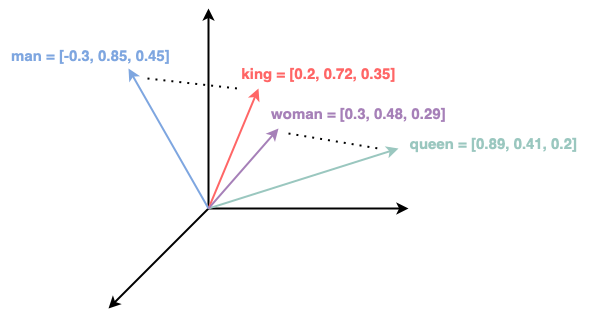
\includegraphics[width=\textwidth]{word_embedding}
	\caption{Vārdlietojuma kartējums vektora telpā \cite{BaeldungEmbedding} }
	\label{fig:wordembedding}
\end{figure}

Vārdlietojuma kartējums ļauj arī veikt dažādas operācijas ar vārdiem vektoru telpā, to skaitā arī  saskaitīšanu un atņemšanu. Piemēram, "karalis - vīrietis + sieviete" varētu izveidot vektoru, kas vektora telpā ir tuvu vārdam "karaliene".

\subsection{Pazīmju izvēle}
Iepriekš tika apskatīts kā atlasīt pazīmes no dokumentu kopas. Atkarībā no apskatīto tekstu daudzuma un sarežģītības, rezultātā var tikt iegūts liels pazīmju skaits, kas var apgrūtināt mašīnmācīšanās algoritmu pielietošanu. Pārāk plaša vai pārāk maza pazīmju kopa var atstāt negatīvu iespaidu uz modeļa veiktspēju. Lai risinātu šo problēmu tiek apskatīta pazīmju izvēle.

Viena no izplatītākajām metodēm, kas samazina pazīmju skaitu ir retu vārdu izņemšana. Dēļ to retuma, tās visdrīzāk nav pazīmes, kas ir raksturīgas visiem kategoriju tekstiem, un nepalīdzēs izveidot precīzāku modeli.

\section{Biežākās problēmas tekstu klasifikācijā}
\subsection{Vārdu neskaidrība}
 Dabiskā valoda ir būtībā neskaidra, ar vārdiem un frāzēm, kuriem ir vairākas nozīmes atkarībā no konteksta. Šīs neskaidrības precīza risināšana ir izaicinājums teksta klasifikācijas modeļiem.

\subsection{Tekstu nevienmērība}
Teksta dati ir dažādi un atšķiras pēc garuma, struktūras un kvalitātes. Tie var ietvert rakstos raksturīgas kļūdas, slengu, saīsinājumus un plašu rakstīšanas stilu klāstu, kas padara tos grūti standartizējamus.

\subsection{Pārmērīga pielāgošana}
Pārmērīga pielāgošana nozīmē to, ka klasifikators ir pārāk labi modelējis apmācības datus
un nedarbojas labi uz iepriekš neredzētiem datiem. Kļūdas, ko klasifikators pieļauj uz apmācības datiem sauc par apmācības kļūdām, savukārt kļūdas, kuras tiek pieļautas uz iepriekš neredzētiem datiem, sauc par vispārināšanas kļūdām. Labam modelim ir gan zems apmācības kļūdu skaits, gan zems vispārināšanas kļūdu skaits. Nepietiekama pielāgošana notiek ja modelim ir gan augsts apmācības kļūdu skaits, gan arī augsts vispārinājuma kļūdu skaits. No otras puses - pārmērīga pielāgošana notiek kad modelim ir zems apmācības kļūdu skaits, bet augsts vispārināšanas kļūdu skaits \cite{tan2005introduction}. Zemāk apskatāmajā attēlā \ref{fig:pielagosana} attēloti piemēri divdimensiju klasifikācijas scenārijā.

\begin{figure}[H]
	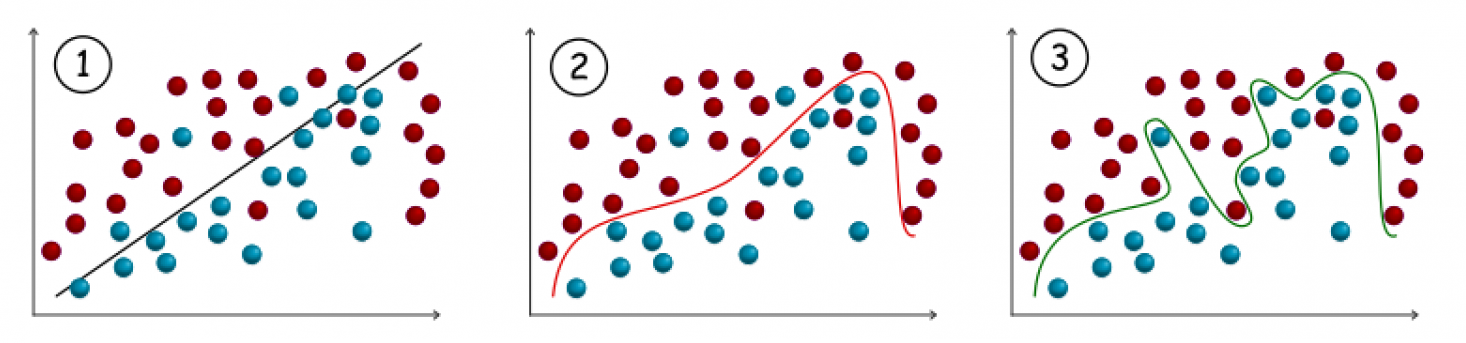
\includegraphics[width=\textwidth]{pielagosana}
	\caption{Pielāgošanas scenāriji (1 - nepietiekama, 2 - optimāla, 3 - pārmērīga)}
	\label{fig:pielagosana}
\end{figure}
 
Visbiežāk šāda veida kļūdas rodas no apmācību datiem, kuros ir pārāk daudz ar konkrēto klasifikāciju nesaistīti dati (lieks fona “troksnis”) vai arī izvēlētais apmācību datu apjoms ir pārāk mazs.

\newpage
\section{Mašīnmācīšanās rīki}
\subsection{scikit-learn}
Viena no Python valodas populārākajām mašīnmācīšanās bibliotēkām, kas palīdz risināt problēmas kā klasteru veidošana, regresija, klasifikācija, dimensiju skaita samazināšana, ir ‘sckit-learn’. Sākotnēji bibliotēku izstrādājis Dāvids Kornepū (David Cournapeau) 2007. gadā, tomēr ātri vien projekts ir izaudzis par atvērtā pirmkoda projektu kuru uztur vairāki simti izstrādātāju.  Bibliotēku izmanto daudzi lieli uzņēmumi kā J.P. Morgan, Spotify u.c. Autors ir izvēlējies lietot šo bibliotēku lai atvieglotu plaši lietotu klasifikācijas algoritmu implementāciju (Naivā Bejesa metode, loģistiskā regresija, lēmumu koki,  atbalsta vektoru mašīnas). 
\subsection{Tensorflow}
TBD
